%! TeX program = lualatex
%---------------------------ALLGEMEINE IMPORTS-------------------------------------
\documentclass[12pt,english,ngerman]{scrartcl}

\usepackage{iftex}

% text input and font
\ifluatex  % LuaLaTeX
    \usepackage{fontspec}
    % main font automatically: Latin Modern
    %\setmonofont{Consolas}
    % \newfontfamily{\Consolas}{Consolas}
\else  % pdfLaTeX
    \usepackage[utf8]{inputenc}  % input in UTF-8
    \usepackage[T1]{fontenc}  % output in T1 fonts (west European encoding)
    \usepackage{lmodern}  % Latin modern font for main text
    \usepackage[mono]{zi4}  % Consolas font for monospaced text
    % \newfontfamily{\Consolas}{\fontfamily{zi4}}
\fi

% text processing
\usepackage{babel}  % language package
\usepackage[intlimits]{mathtools}  % upgrade of amsmath (automatically loaded) - \int^_ like \limits^_
\usepackage{amssymb}  % upgrade of amsfonts (American Math Society)
\usepackage{amstext}  % \text command in math environments
%\usepackage{bm}  % bold math fonts
% \LetLtxMacro{\svqty}{\qty}
% \usepackage{physics}  % macros for easier typesetting of physical formulas
% \LetLtxMacro{\qty}{\svqty}
\usepackage{letltxmacro}  % \let command for robust macros (new sqrt)
\usepackage{chemformula}  % typeset chemical formulas
\usepackage{microtype}


% page geometry
\usepackage{scrlayer-scrpage}  % page formatting with KOMA options
\usepackage[paper=a4paper, hmargin=3cm, vmargin=2.5cm, includehead, includefoot, head=29pt]{geometry}  % horizontal: 3cm, vertical: 2.5cm strict with or without headers and footers
\usepackage{tabto}  % tab stops
\NumTabs{8}  % 8 equally spaced of \textwidth tab stops



% floats
\usepackage[hypcap=false, labelfont=bf]{caption, subcaption}  % caption editing - hypcap warning with hyperref
\usepackage{float}  % for [H] (forced here) specifier
\usepackage{tabularray}
\usepackage{diagbox}  % table cells with diagonal lines


% graphical input
\usepackage{graphicx}  % input JPEG, PNG, PDF, etc.
\usepackage{pdfpages}  % input PDF as whole pages
\usepackage{lastpage}  % reference to last page
\usepackage{pgfplots}  % for tikzplotlib
\usepgfplotslibrary{groupplots,dateplot}
\usetikzlibrary{patterns,shapes.arrows}
\pgfplotsset{compat=newest}
\usepackage{import}


% text
\usepackage[locale=DE, uncertainty-mode=separate]{siunitx}  % SI units, German formatting - \pm stays \pm instead of ..(.)
\let\svqty\qty %dont import physics before siunitx is loaded
\usepackage{physics}
\let\qty\svqty
\usepackage{icomma}  % no space after commas instead of English points) in decimal values
\usepackage{enumitem}  % better enumerating with style options
\usepackage{nicefrac}  % inline-fractions in n/d-style
\usepackage{xcolor}  % custom colors
\usepackage{listings, scrhack}  % code display; listings in combination with KOMA
\usepackage{fancyvrb}  % Verbatim environment with better options (capital V!)

\usepackage{listings}

% literacy
\usepackage[bibencoding=auto,backend=biber,autolang=other]{biblatex}  % backend=Biber is standard
\usepackage{csquotes}  % better quotation - should also be used in combination with package babel (warning)
\usepackage{xurl}  % breaks links - after BibLaTeX, but before hyperref!
\usepackage[hidelinks]{hyperref}  % produces most errors, last to load
\usepackage{bookmark}


% KOMA setups
% header and footer
\pagestyle{scrheadings}  % KOMA style
\clearpairofpagestyles  % reset
\setkomafont{pageheadfoot}{\normalfont}  % standard font in header and footer
\setlength{\headheight}{29pt}  % just look at the warning
\cfoot{\pagemark{} / \pageref*{LastPage}}  % center foot - *: ref but no hyperlink
% {}: empty statement
% \ : protected space
% \,: small space
\DeclareTOCStyleEntry{dottedtocline}{section}  % sections in TableOfContents with dotted lines
\KOMAoptions{parskip=half-}  % paragraphs with half a line height space instead of indentation, last line with no special treatment


% package setups

% biblatex
%\addbibresource{files/JabRef_Database/physics.bib}
% \addbibresource{transistor.bib}

% rewrite names (babel overwrites German with standard English names, therefore at document beginn [after everything is loaded])
\AtBeginDocument{\renewcommand{\refname}{Literaturverzeichnis}}
% others:
% \contentsname
% \listtablename
% \listfigurename


% xcolor
\definecolor{code_keyword}{HTML}{A06E9D}
\definecolor{code_string}{HTML}{AD6E3E}
\definecolor{code_comment}{HTML}{6A9955}
%\definecolor{code_basic}{HTML}{D4D4D4}
%\definecolor{code_background}{HTML}{1E1E1E}

% siunitx
\DeclareSIUnit{\dig}{dig}  % digits for uncertainty of electronical measurement devices
\sisetup{locale = DE}  % deutschsprachige SI-Konvention
\sisetup{per-mode = fraction}
\DeclareSIUnit{\px}{px}
\DeclareSIUnit{\strich}{|||}

%Eigene Commands
\newcommand{\der}[2]{\frac{\mathrm{d}#1}{\mathrm{d}#2}}
\newcommand{\pder}[2]{\frac{\partial #1}{\partial #2}}

% listings
\lstdefinestyle{python}{
    %basicstyle=\Consolas\footnotesize,%\color{code_basic},  % \footnotesize contains \selectfont implicitly
    %backgroundcolor=\color{code_background},
    commentstyle=\color{code_comment},
    keywordstyle=\bfseries\color{code_keyword},
    numberstyle=\tiny,
    stringstyle=\color{code_string},
    breakatwhitespace=false,
    breaklines=true,
    captionpos=b,
    keepspaces=true,
    numbers=left,
    numbersep=5pt,
    showspaces=false,
    showstringspaces=false,
    showtabs=false,
    tabsize=2,
}
\lstset{style=python}
\ifPDFTeX
    \renewcommand*{\ttdefault}{lmvtt}  % Latin Modern Typewriter Proportional
\fi


% new sqrt
% https://en.wikibooks.org/wiki/LaTeX/Mathematics
\makeatletter
\let\oldr@@t\r@@t
\def\r@@t#1#2{%
    \setbox0=\hbox{$\oldr@@t#1{#2\,}$}\dimen0=\ht0
    \advance\dimen0-0.2\ht0
    \setbox2=\hbox{\vrule height\ht0 depth -\dimen0}%
    {\box0\lower0.4pt\box2}}
\LetLtxMacro{\oldsqrt}{\sqrt}
\renewcommand*{\sqrt}[2][\ ]{\oldsqrt[#1]{#2} }
\makeatother


% own commands
% \newcommand* can't contain multiple lines
% \newcommand can
\newcommand*{\mup}[1]{\ensuremath{\text{\textup{#1}}}}  % upright normal font in math mode
\newcommand*{\inkgraphics}[3][\linewidth]{\def\svgwidth{#1}\import{#2}{#3}}


% tabularray
% imports_and_setups{
%     expl3,
%     xparse,
%     ninecolors
%     \hypersetup{pdfborder={0 0 0}}
% }

% tabularray environments
\RequirePackage{tabularray}  % like \usepackage but for packages
\UseTblrLibrary{siunitx}  % siunitx suited for tabularray
\UseTblrLibrary{bookmark}  % bookmark suited for tabularray
% TRIPLE BRACKETS {{{}}} to protect strings from \num{} interpretation in S columns
\UseTblrLibrary{diagbox}  % diagbox suited for tabularray
\UseTblrLibrary{varwidth}  % measure cell width using package 'varwidth'

% standard environment
\SetTblrInner{
    hlines,
    vlines,
    columns={
            halign=c,
            valign=m,
        },
    measure=vbox,
}

% X columns
\NewTblrEnviron{tblrx}
\SetTblrInner[tblrx]{
    hlines,
    vlines,
    columns={
            halign=c,
            valign=m,
            co=1,  % coefficient of width for expendable columns (X columns)
        },
    width=\linewidth,
    vspan=minimal,
    measure=vbox,
}

% -X columns
\NewTblrEnviron{tblr-x}
\SetTblrInner[tblr-x]{
    hlines,
    vlines,
    columns={
            halign=c,
            valign=m,
            co=-1,  % shrinks X column down to natural width
        },
    width=\linewidth,
    vspan=minimal,
    measure=vbox,
}

% no hline and vline left and on top of first cell
\NewTblrEnviron{tblr_omit_first_cell}
\SetTblrInner[tblr_omit_first_cell]{
    hlines,
    vlines,
    columns={
            halign=c,
            valign=m,
        },
    hspan=even,
    vspan=minimal,
    %
    hline{1}={1}{white},  % first row, only first cell
    vline{1}={1}{white},
    measure=vbox,
}


\addbibresource{cmos.bib}
    % Kopfzeile
\ihead{SS22\\18.05.2022}
\chead{\textsc{Hinterleitner} Michael - 12002411 \\ \textsc{Philipp} Maximilian - 11839611}
\ohead{LU ECM-\\ CMOS Logik}
    % Fußzeile
%--------------------------------------AB HIER DOKUMENT---------------------------------------------
\begin{document}
% 
\includepdf{deckblatt2.pdf}
\tableofcontents
\newpage


%\section{Aufgabenstellung}\label{sec:Aufgabenstellung}

% Die nachfolgende Aufgabenstellung wurde von den Laborbetreuern bereitgestellt
% und beinhaltet sowohl Angaben zur Vorbereitung als auch zur praktischen
% Durchführung der Übung:

% zu 1: Aufgabenstellung Das vor der Übung verteilte Aufgabenblatt.
 
\includepdf[
     pages=-,  % all pages
     addtotoc={
         1, section, 1, Aufgabenstellung, sec:Aufgabenstellung
     }
 ]{angabe.pdf}

% zu 2: Vorbereitung Es sind beide Vorbereitungen dem Protokoll beizufügen.
% \section{Vorbereitung}\label{sec:Vorbereitung}
%Die folgende Vorbereitung wurde vor der Laborübung 
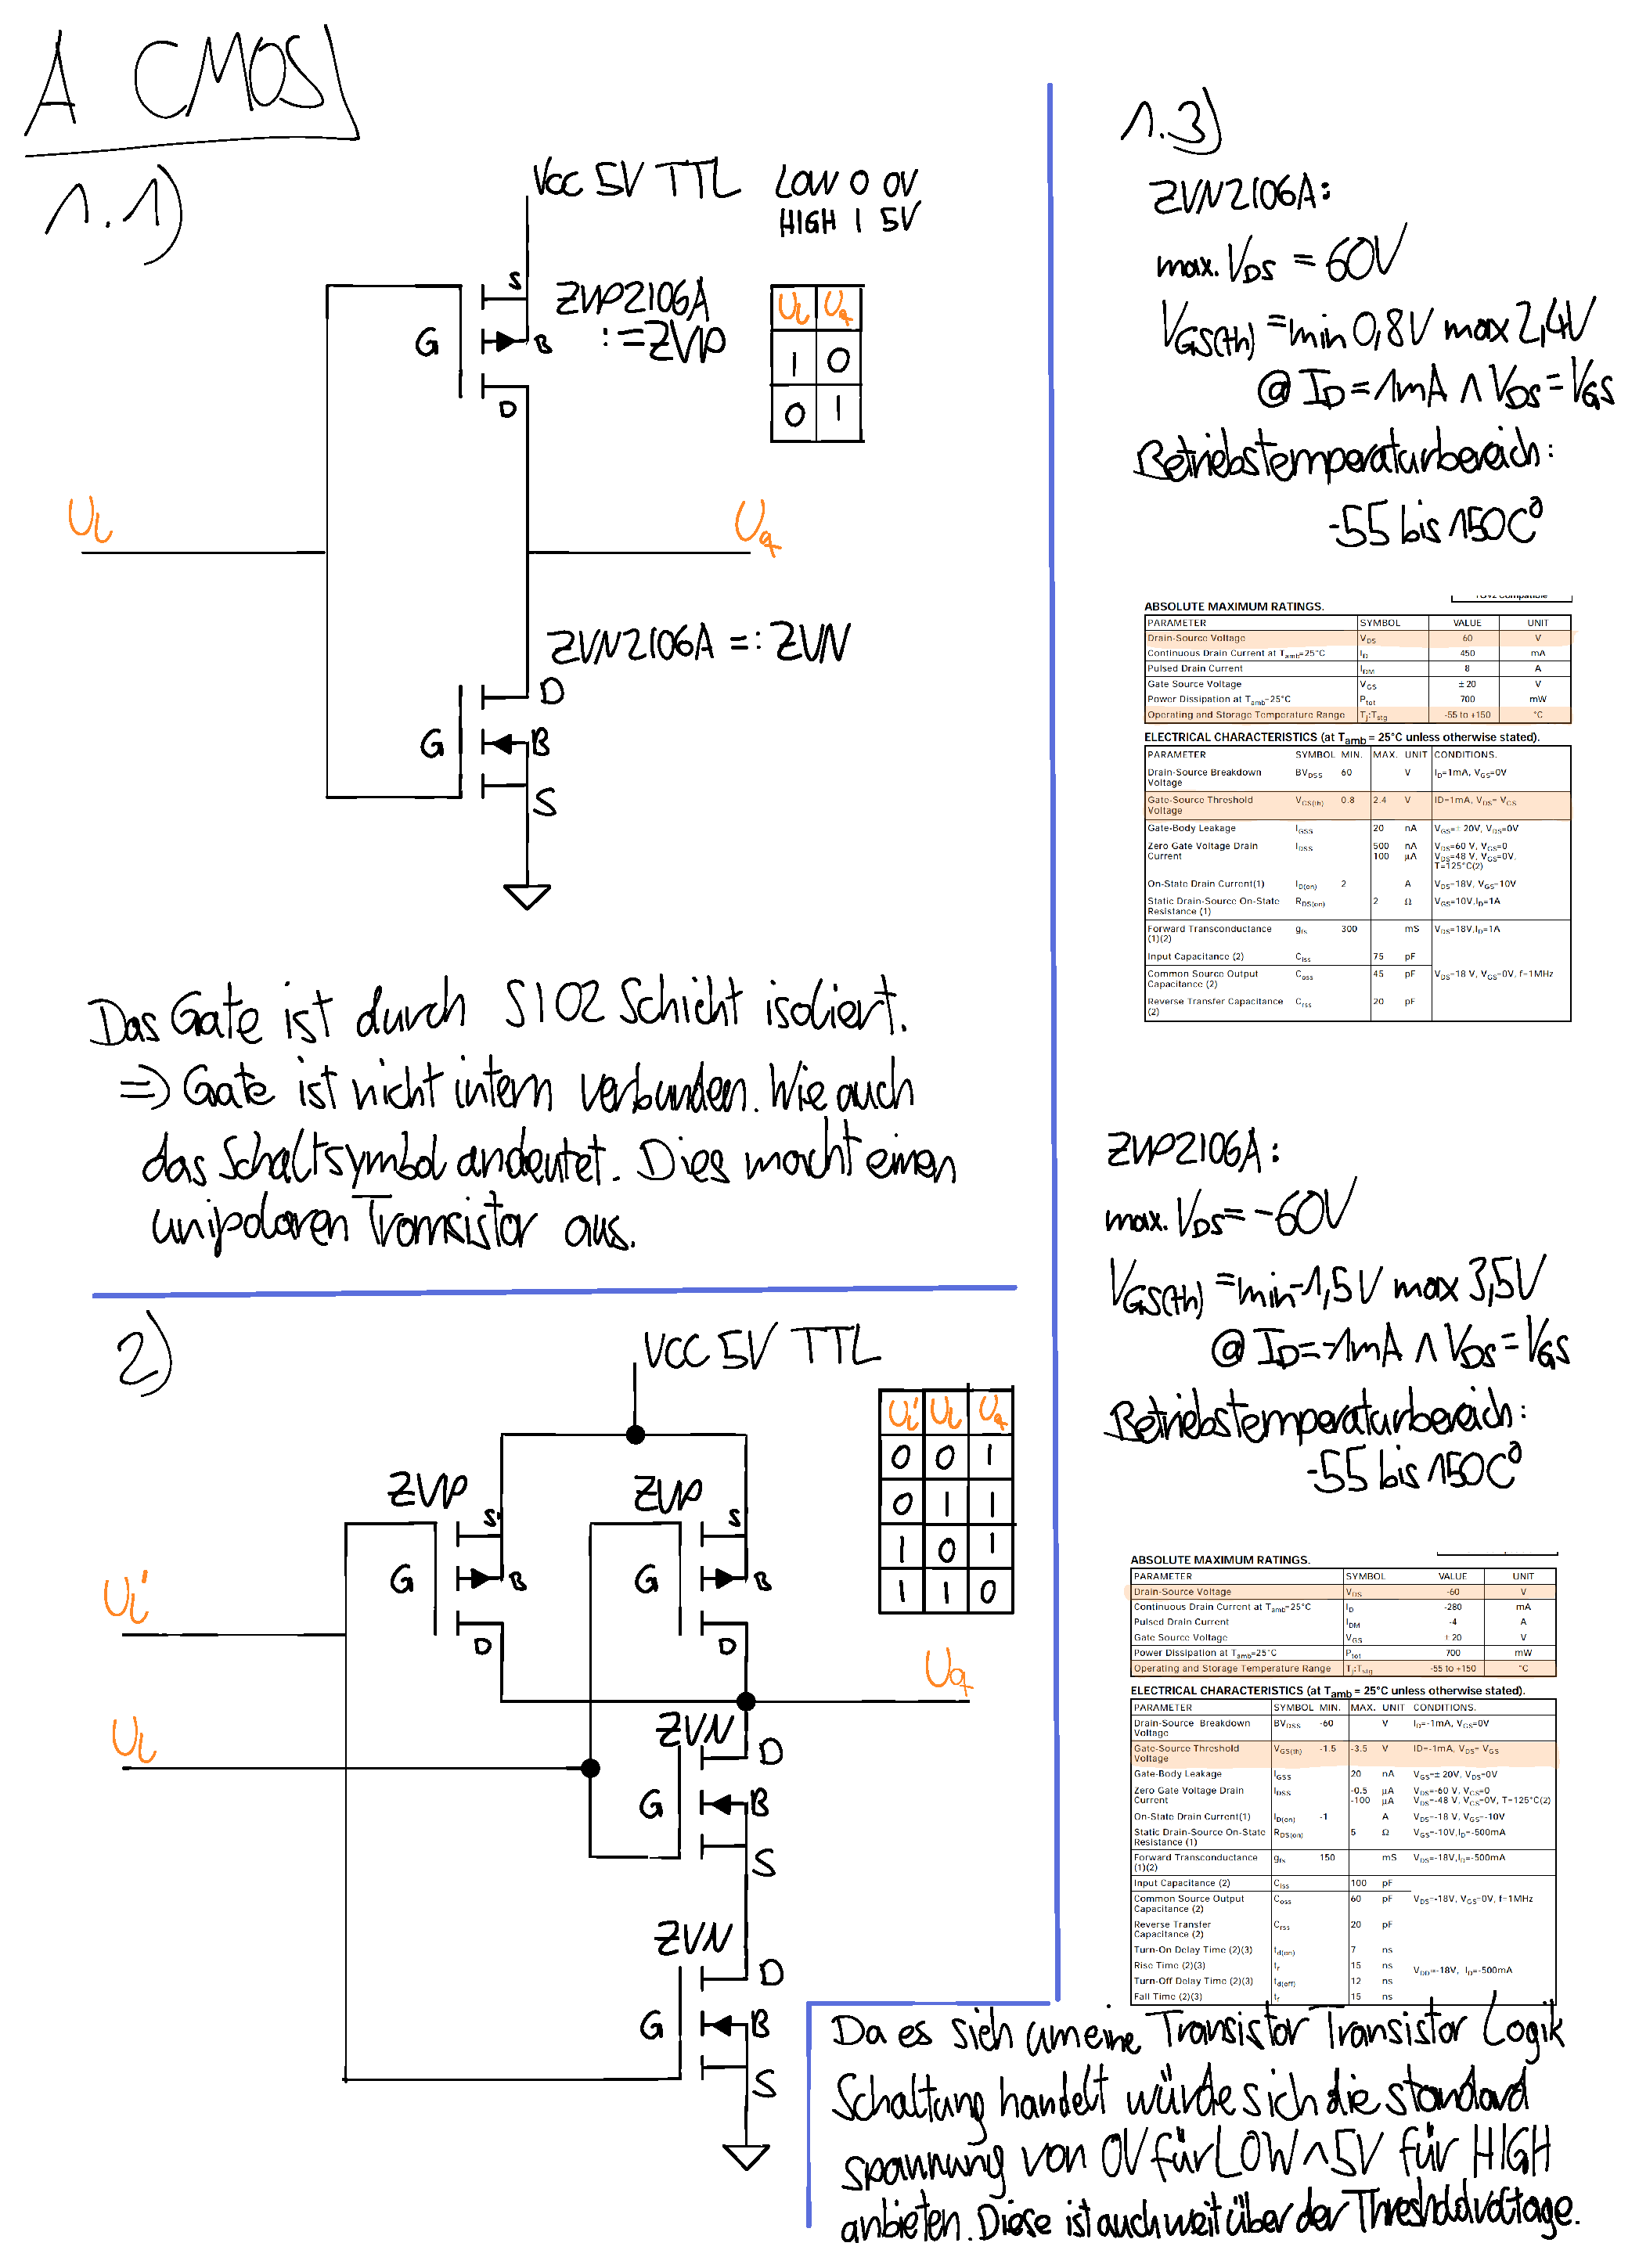
\includepdf[pages=-,
     addtotoc={
         1, section, 2, Vorbereitung, sec:Vorbereitung
     }]{./figures/CMOS-Logik1.pdf}
\includepdf[pages=-]{./figures/CMOS-Logik2.pdf}
% 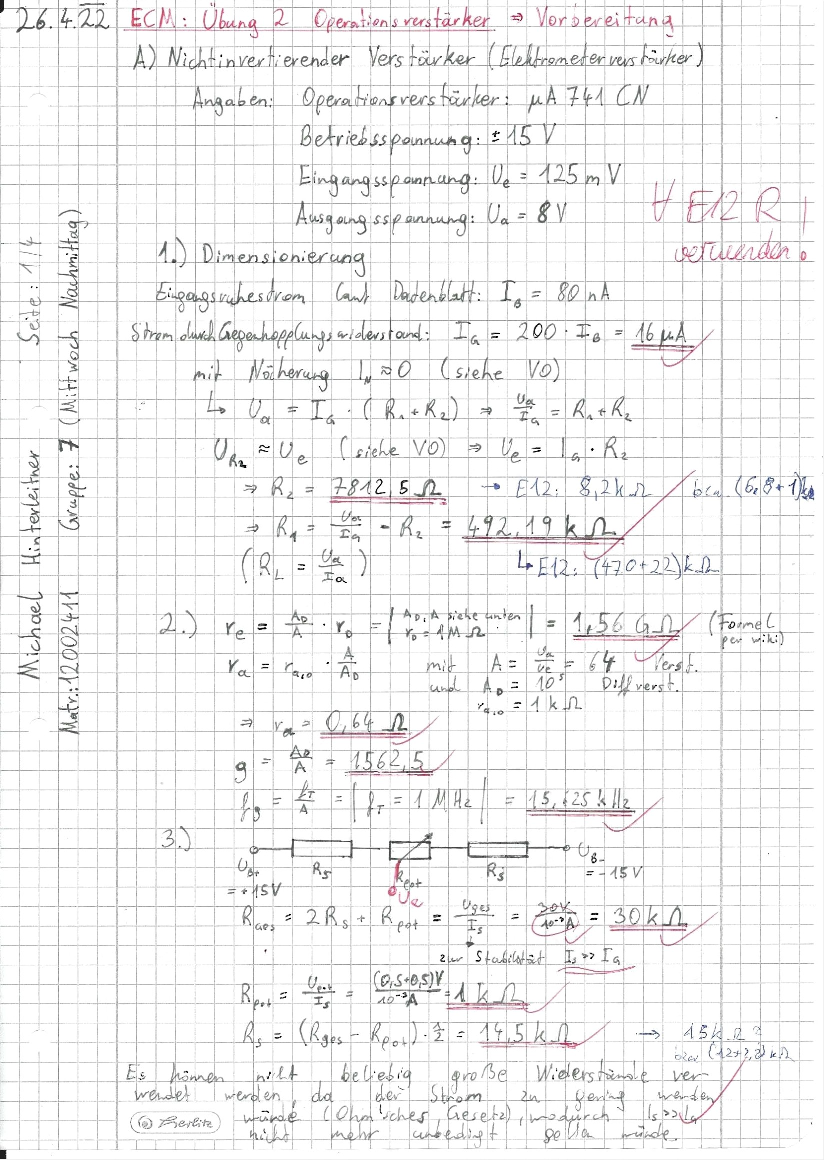
\includepdf[pages=-]{./mh_vorbereitung_opv.pdf}


% zu 3: Grundlagen In den Grundlagen sollen die später verwendeten Formeln
% stehen und kurz erklärt werden, dabei ist es nicht notwendig Formeln
% herzuleiten. Quellenangaben sind an dieser Stelle von Vorteil, weil Sie so
% schnell die betreffenden Stellen in Unterlagen finden. In den Rechnungen
% werden grundlegende Annahmen skizziert und begründet und dann mit diesen
% Annahmen, die für die Schaltungen notwendigen Werte berechnet. Dabei kann
% auch gleich auf die später wirklich verwendeten Werte Bezug genommen werden -
% wir verwenden bei den Widerständen zum Beispiel von den Normwert-Reihen die
% E12 und/oder E24 Serie (nach DIN 41426 bzw. IEC 63).
\section{Grundlagen}\label{sec:Grundlagen}
%in Grundlagen
Operationsverstärker (kurz 'OPV oder 'OpAmp') dienen grundlegend der Verstärkung von 
Gleichspannungen. Sie besitzen einen nicht-invertierenden, der meist mit einem 
Plus, und einen invertierenden Eingang, der mit einem Minus dargestellt wird. Zu 
beachten ist, dass die Verstärkung auf die Differenzspannung der beiden Eingänge 
wirkt. Je zwei zusätzliche Anschlüsse finden sich für die positive und negative 
Betriebsspannung und für den Offsetabgleich, damit bei keiner Eingangsspannung 
auch keine Ausgangsspannung auftritt - dieser wird also in einer externen 
Schaltung durchgeführt.

\begin{figure}[H]
    \centering
    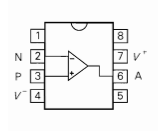
\includegraphics[width=6cm, height=6cm,keepaspectratio]{./figures/pics/pins.PNG}
    \caption{Schematische Darstellung der Pinbelegung eines klassischen Operationsverstärkers. Hierbei bezeichnet 2 den invertierenden, 3 den nicht-invertierenden Eingangskanal, 6 den Ausgang, 4 den Anschluss für die negative sowie 7 den Anschluss für die positive Betriebsspannung, 1 und 5 die Pins für den Offsetabgleich und 8 einen freien Pin.  \cite{tietze}}
    \label{fig:pin_anschl}
\end{figure}

In \autoref{fig:pin_anschl} sind die Pins eines Operationsverstärkers, wie er auch 
in der Laborübung verwendet wurde, zu sehen. Dabei ist zu beachten, dass jeder nicht 
belegte Pin auf Masse gelegt werden soll.

Es gibt vier grundlegende Arten der Verwendung von Operationsverstärkern, darunter
der nicht-invertierende Betrieb, bei dem das Eingangssignal nur auf den nicht-invertierenden 
Kanal gelegt wird und der invertierende auf Masse gelegt wird. Analog funktioniert der invertierende 
Modus, bei dem das Signal anstelle nun an den invertierenden Eingang gelegt wird, wodurch die Ausgangsspannung 
zusätzlich zur Verstärkung noch zum Eingangssignal invertiert wird. Beim Differenzbetrieb werden an 
beide Eingänge Signale angelegt und die Differenzspannung verstärkt. Im Falle des Gleichtaktbetriebs 
liegt das gleiche Eingangssignal an den beiden Eingängen an, wodurch es theoretisch keine Differenzspannung 
und Verstärkung geben sollte - in der Realität resultiert allerdings eine Verstärkung, die als 
Gleichtaktverstärkung bezeichnet wird.

Da der Operationsverstärker ohne zusätzliche Verkopplung sehr stark frequenzabhängig ist und 
nur eine geringe Bandbreite gewünscht verstärkt, wird eine Gegenkopplung vom Ausgang zum Eingang 
durchgeführt, wodurch die Verstärkung zwar abnimmt, die Bandbreite jedoch stark vergrößert wird. 
Die Bandbreite wird wie gewohnt durch die Grenzfrequenz charakterisiert, bei welcher die Verstärkung 
noch \SI{70}{\%} der maximalen beträgt. Wenn nun beispielsweise ein Kondensator in der Rückkopplung verbaut wird, 
handelt es sich um eine Integratorschaltung, die im zweiten Teil der Laborübung untersucht wird.

Die resultierende Verstärkung lässt sich gemäß \autoref{eq:ver} als Verhältnis der Ausgangs- $U_a$ zur Eingangsspannung $U_e$ berechnen.
\begin{equation}
	V=\frac{U_a}{U_e}
	\label{eq:ver}
\end{equation}


% zu 4: Versuchsdurchführung In diesem Punkt wird die Durchführung der
% einzelnen Aufgaben beschrieben. Im Simulationsteil ist die simulierte
% Schaltung mit allen Analyseparametern darzustellen. Im praktischen Teil sind
% die verwendete Geräte sowie die gemessenen Werte der verwendeten Bauteile
% anzugeben. Außerdem sind durchgeführte Funktionsüberprüfungen der Bauteile
% (Dioden, Transistor, etc.) anzuführen. Die Messergebnisse bzw. Oszillogramme
% sind mit Angabe der verwendeten Messgeräte anzugeben. Oszillogramme werden
% vom verwendeten Oszilloskop als Daten auf einen USB-Stick ausgegeben und
% können in das Protokoll aufgenommen werden. Das gleiche gilt für Schaltungen
% bzw. Ergebnissen von Simulationen. Es ist auf eine klare Darstellung der
% Messergebnisse und –auswertung zu achten (Tabellen, geeignete Grafiken). Die
% originalen, während des Versuchs angefertigten Aufzeichnungen sind dem
% Protokoll beizufügen. 
\section{Versuchsdurchführung}\label{sec:versuchsdurchfuehrung}
Für den praktischen Teil an der Steckplatine wurden Widerstände der E12-Reihe,
mit denen die in der Vorbereitung angegebenen respektive errechneten Werte
angenähert wurden, verwendet. 

Die verwendeten Geräte sind \autoref{tab:geraeteliste} zu entnehmen.

\begin{table}
  \caption{Tabelle der verwendeten Geräte}
  \label{tab:geraeteliste}
  \centering
  \begin{tabular}{l|l}
    \hline
   \multicolumn{2}{ c }{\textbf{Geräteliste}} \\
    \hline
    \textbf{Gerät/Bauelement} & \textbf{Typ} \\
    \hline
    Oszilloskop & \textit{Tektronix TDS 2002}\cite{oszilloscope}\\
    Funktionsgenerator & \textit{H-TRONIC FG250D}\cite{funktionsgenerator} \\
    Netzgerät & nicht bestimmbar\\
    Multimeter & \textit{Fluke 175 TrueRMS}\cite{fluke175} \\
    % todo references
    N-MOSFET & \textit{ZVN2106A}\\
    P-MOSFET & \textit{ZVP2106A}\\
    NOT-Gatter & \textit{74LS04}\\
    2x-NOR-Gatter & \textit{74LS02}\\
    3x-NOR-Gatter & \textit{74LS27}\\
    \hline
  \end{tabular}
\end{table}

\paragraph{Entprellter Schalter}
%TODO text erklaeren wie der Schalter angesteuert wird und wo er verwendet wurde
Der entprellter Schalter wird als Signalgeber für die logischen Schaltungen und
Gatter verwendet. Der Aufbau dieses Schalters ist in
\autoref{fig:aufbau_schalter} ersichtlich, jedoch ist noch der \textit{GND} mit
Ground und \textit{VCC} mit \SI{5}{\volt} zu beschalten damit das Signal von
Schalter eins bzw Schalter zwei von den jeweiligen Betriebsart abgegriffen
werden.

Jeder dieser Schalter hat einen Standard \textit{HIGH} bzw.
\textit{LOW} Betriebsart.

\begin{figure}[H]
  \centering
    % 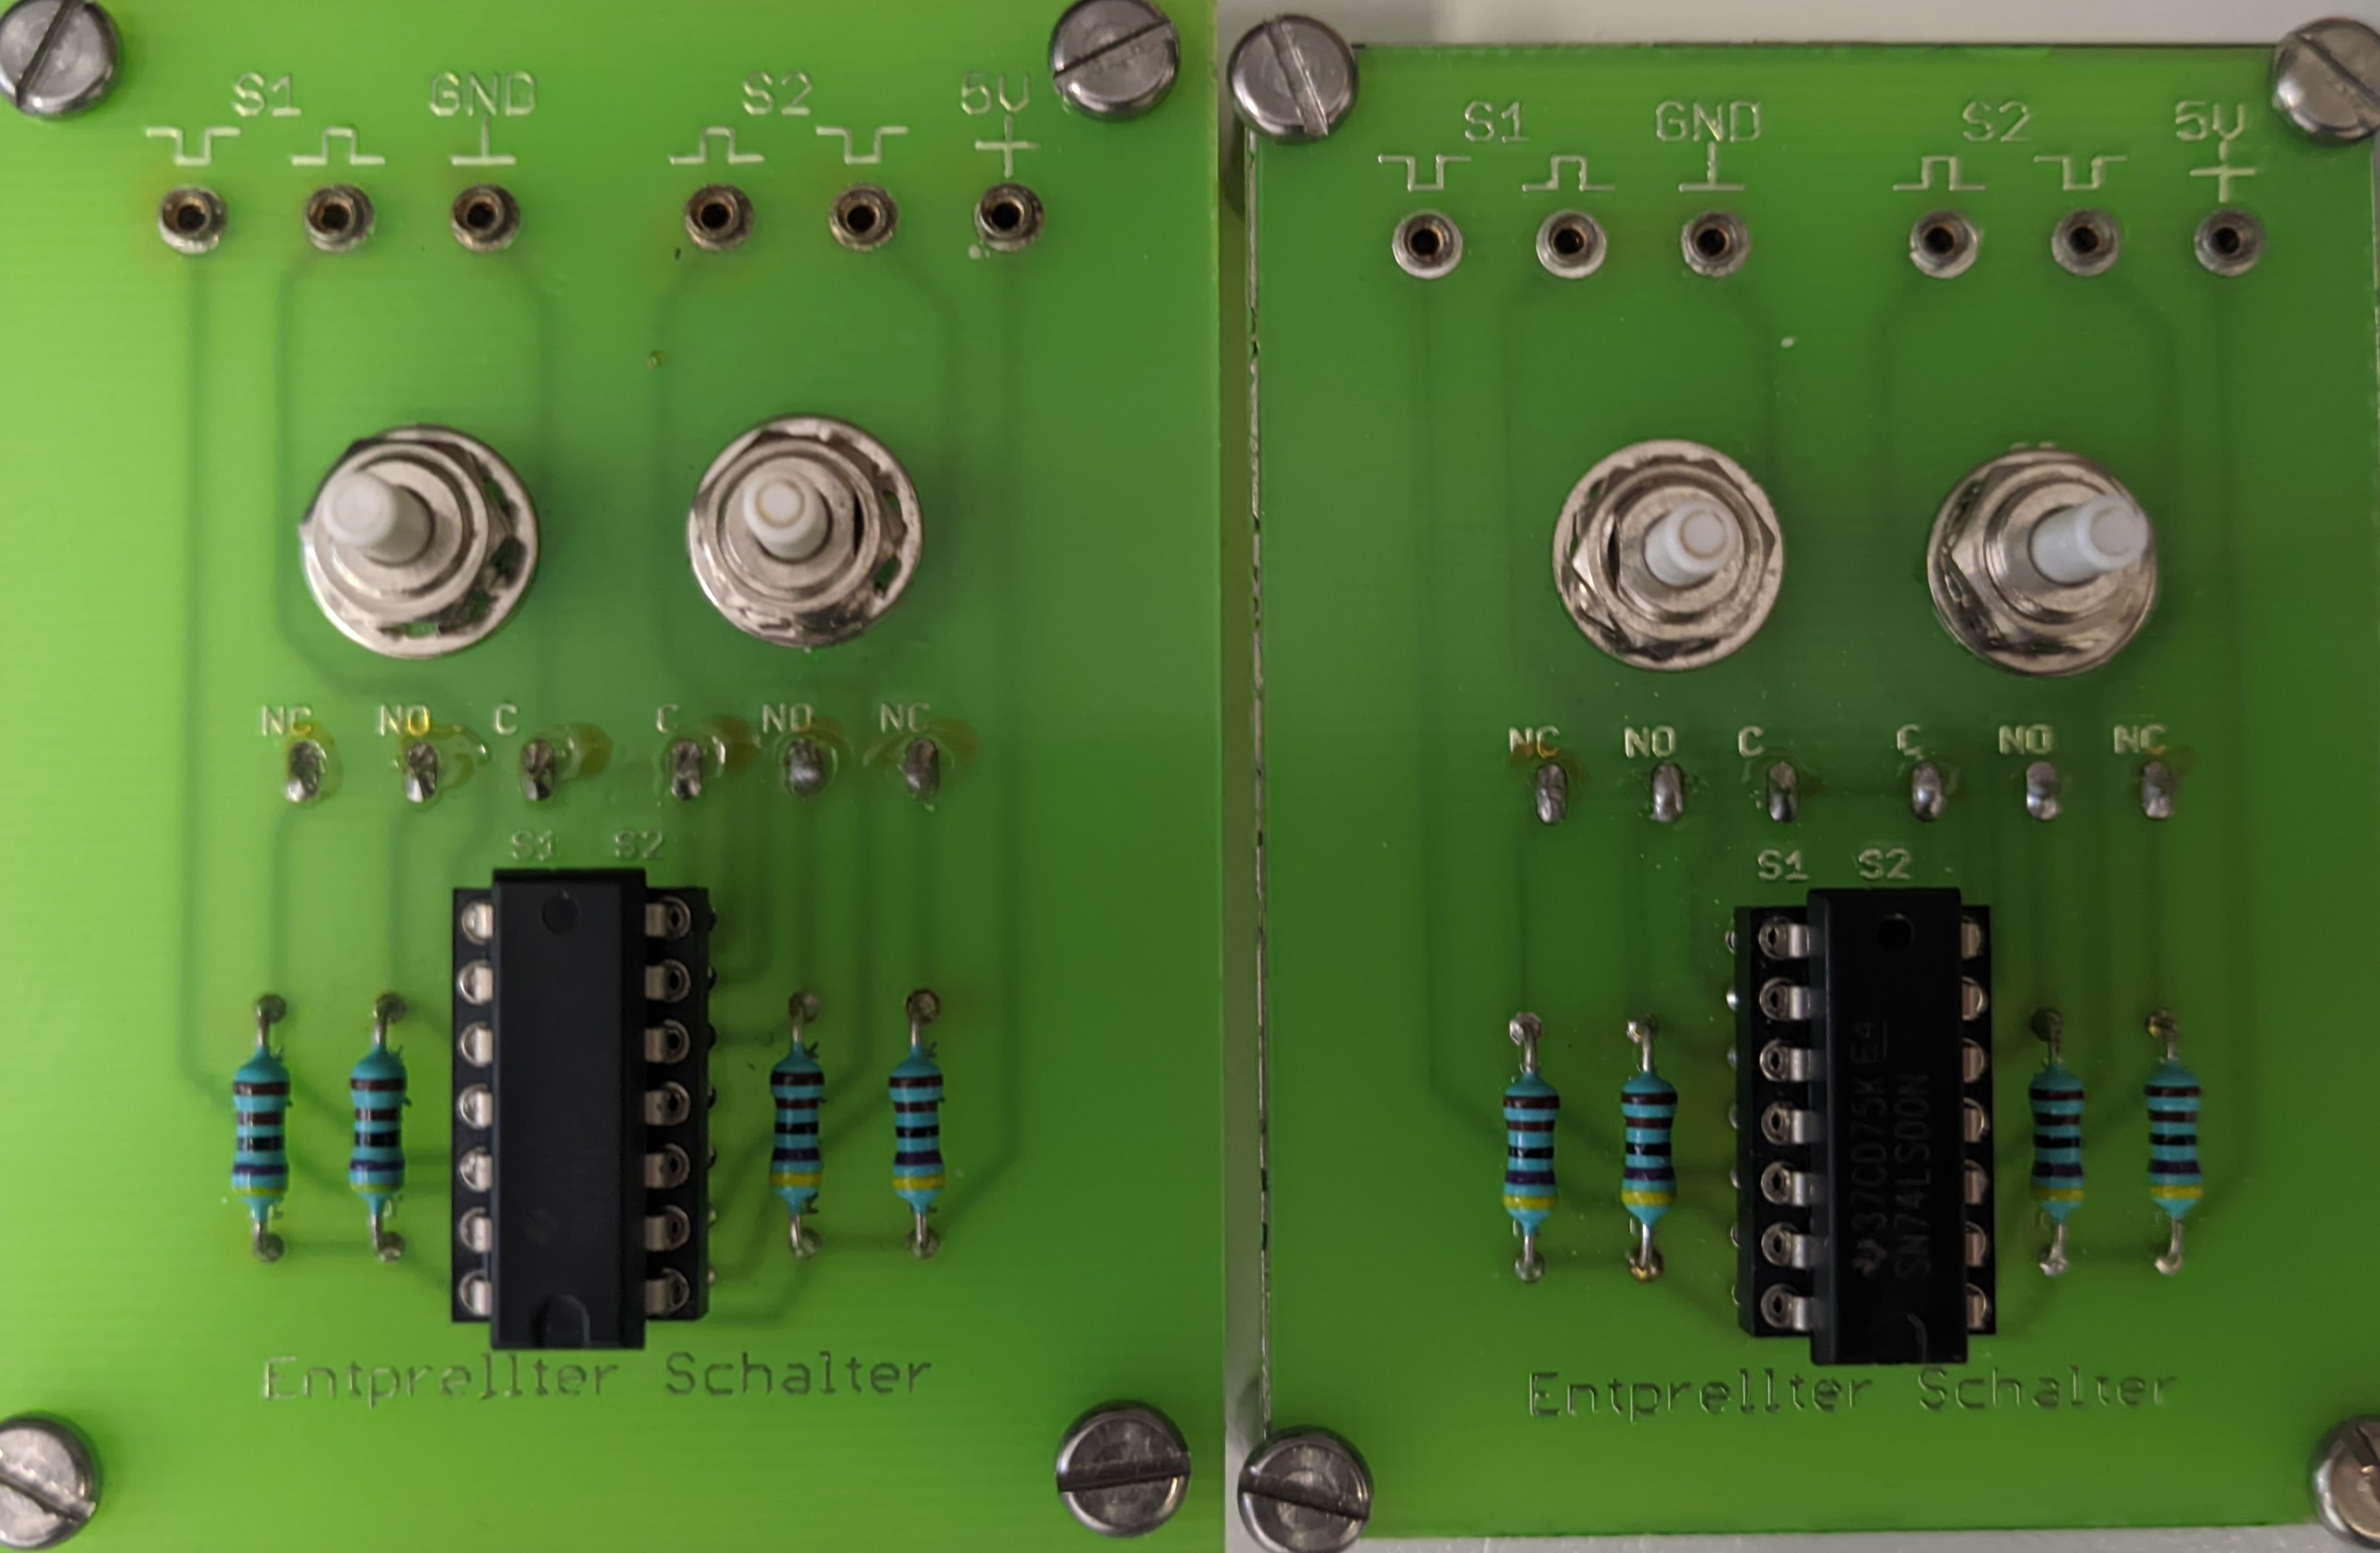
\includegraphics[width=0.95\textwidth]{./figures/messungen/schalter.png}
  \caption{}
  \label{fig:aufbau_schalter}
\end{figure}


\paragraph{LED Leiste}
%TODO text erklaeren wie der Leiste angesteuert wird und wo er verwendet wurde

Damit die Aufnahmen der Schaltungen übersichtlich bleiben wurde diese meistens
von den Aufnahmen weggeschnitten und in der Grafik mittels \textit{LED} oder in
der Beschriftung gekennzeichnet bzw. erwähnt.

\subsection{CMOS}
% Simulation:
\subsubsection{Simulation}
% 2.1
% Die Inverter-Schaltung ist mit LTspice zu simulieren.
\paragraph{Aufbau des CMOS-Inverters}

%TODO text simulation

%TODO figure sim Aufbau
\begin{figure}[H]
  \centering
    % \includegraphics[width=0.95\textwidth]{./figures/messungen/aufbauinverter.pdf}
  \caption{}
  \label{fig:sim_aufbau_inv}
\end{figure}


% Die Übertragungskennlinie
% und die Stromaufnahme sind darzustellen (PULSE-Quelle).
%TODO text messung Wie wurde simuliert wie wurde die Schwellspannung gemessen.

%TODO figure messung
% 2.2
% Die Gate-Source Schwellspannung ist mit jener der Datenblätter zu vergleichen.

% 2.3
% Die Schaltung des  NAND-Gatters ist mit LTspice zu simulieren. Die Ein- und
% Ausgangsspannungen sind darzustellen (PULSE-Quelle).
\paragraph{Aufbau des CMOS-NAND-Gatters}
%TODO text sim aufbau

%TODO figure sim aufbau
\begin{figure}[H]
  \centering
    % \includegraphics[width=0.95\textwidth]{./figures/messungen/aufbauinverter.pdf}
  \caption{}
  \label{fig:sim_aufbau_nand}
\end{figure}

%TODO text messung Wie wurde die verschiedenen logic states geschalten

%TODO figure messung

% Aufbau am Steckboard:
\subsubsection{Steckboard}
% 2.4 Der CMOS-Inverter ist auf dem Steckboard aufzubauen und seine
% Funktionalität zu prüfen. 
\paragraph{Aufbau des CMOS-Inverters}
%TODO text
Zunächst wird der CMOS-Inverter mittels zweier MOSFETs (einem PMOS \cite{} und
einem NMOS \cite{}) wie nach dem Schaltbild (\autoref{fig:sim_aufbau_inv})
aufgebaut. Jedoch wurden zur Visualisierung des Eingangszustands $U_l$ und des
Ausgangszustands $U_q$ LEDs der LED-Leiste parallel dazu geschaltet. Das
Eingangssignal wurde durch einen entprellten Schalter, im Standardzustand
\textit{LOW}, gegeben, der Aufbau genaue kann im \autoref{} gesehen werden. Als
Spannungsquelle wurde einstellbares Netzteil verwendet und auf \SI{5}{\volt}
eingestellt. 

%TODO figure
\begin{figure}[H]
  \centering
    \includegraphics[width=0.95\textwidth]{./figures/messungen/aufbauinverter.pdf}
  \caption{Dies ist der Aufbau einer CMOS-Inverter-Schaltung nach dem
  Schaltplan aus \autoref{fig:sim_aufbau_inv}. Wobei $U_q$ das Ausgangssignal
  der Schaltung ist  und $U_l$ das logische Eingangssignal ist. Der Zustand
  beider kann anhand einer LED in der LED-Leiste abgelesen werden.}
  \label{fig:mess_aufbau_inv}
\end{figure}


%TODO text messung
% Als  Pegelgeber wird  für  das  Steckboard  ein vorhandener  elektronisch
% entprellte  Schalter  (mit  Hilfe  eines RS-Flip-Flops)  verwendet.  Der
% Ein-  und Ausgangszustand  ist  jeweils durch  LEDs  anzuzeigen.  Die
% Funktionalität  der Schaltung ist anhand der LEDs zu zeigen.
%TODO figure messung

\begin{figure}[H]
  \centering
    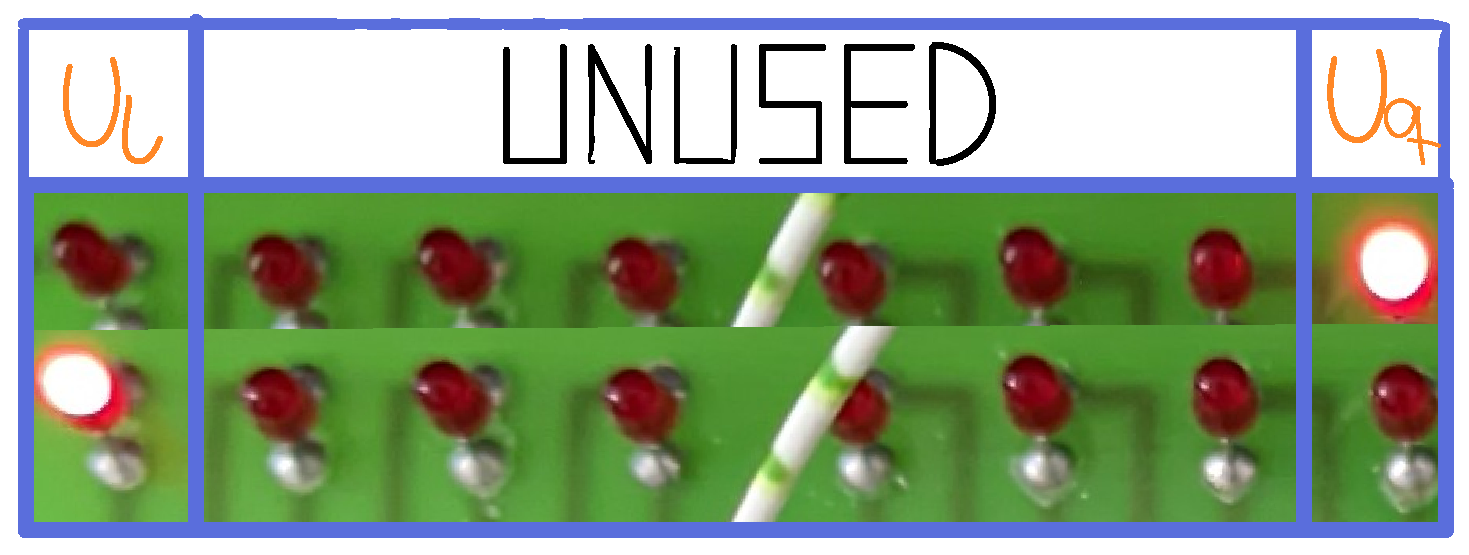
\includegraphics[width=0.95\textwidth]{./figures/messungen/WahrheitstabelleInverter.pdf}
  \caption{}
  \label{fig:mess_wahrheitstabelle_inv}
\end{figure}


% 2.5
% Die Schaltung des  NAND-Gatters ist auf dem Steckboard aufzubauen und ihre
% Funktionalität anhand der LEDs zu zeigen.
\paragraph{Aufbau des CMOS-NAND-Gatters}
%TODO text

%TODO figure
\begin{figure}[H]
  \centering
    \includegraphics[width=0.95\textwidth]{./figures/messungen/aufbaunand.pdf}
  \caption{Dies ist der Aufbau eines CMOS-NAND-Gatters nach dem Schaltplan aus \autoref{fig:sim_aufbau_nand}}
  \label{fig:mess_aufbau_nand}
\end{figure}

%TODO text messung

%TODO figure messung
\begin{figure}[H]
  \centering
    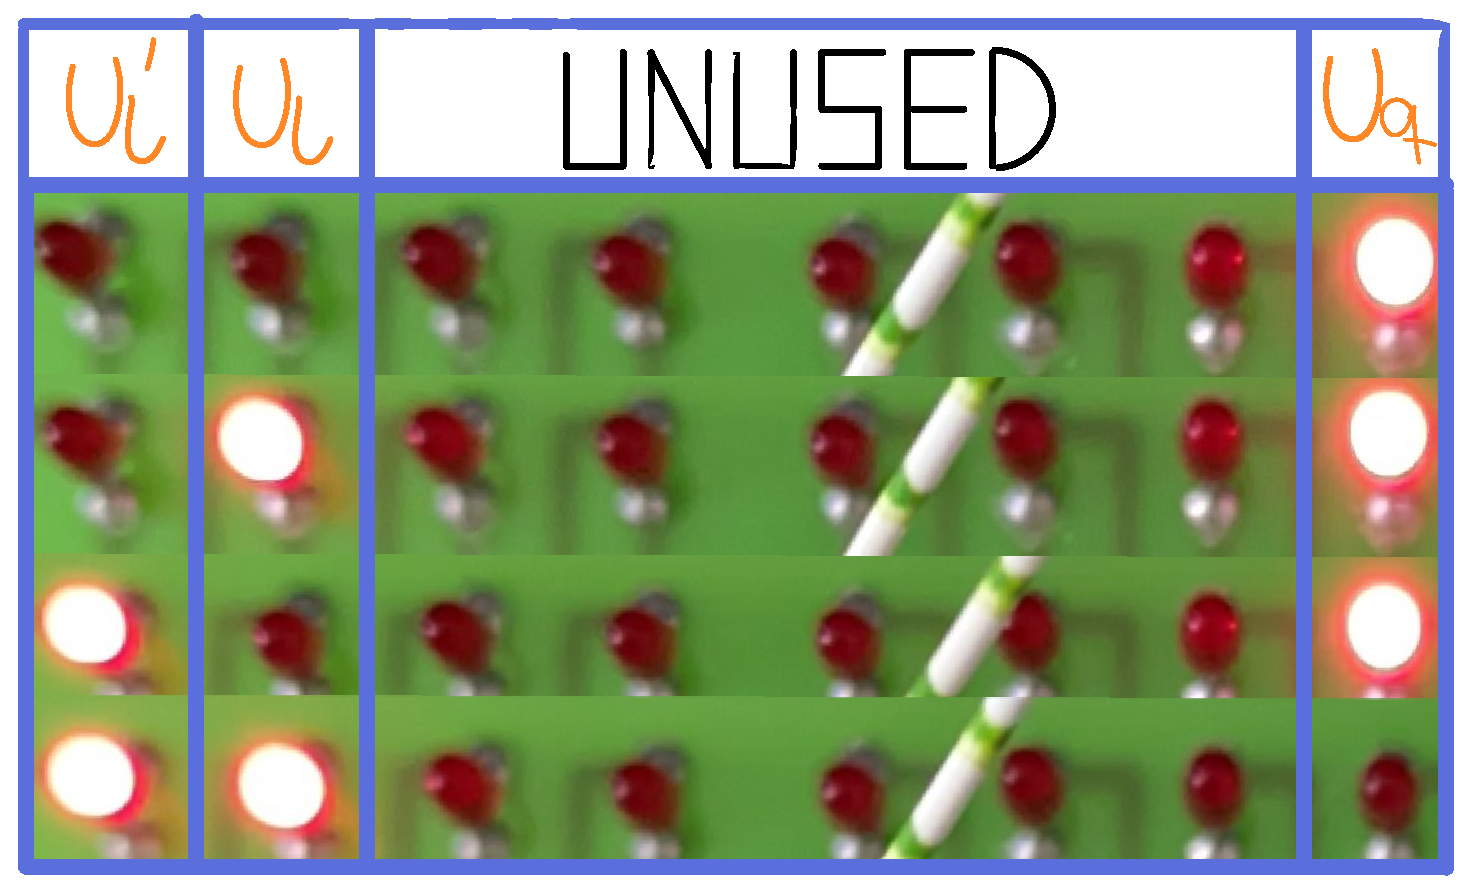
\includegraphics[width=0.95\textwidth]{./figures/messungen/WahrheitstabelleNAND.pdf}
  \caption{}
  \label{fig:mess_wahrheitstabelle_nand}
\end{figure}

% 2.6
% Die Ergebnisse sind zu protokollieren und diskutieren.

\subsection{Schaltungssynthese}
% Simulation:
% 2.1 Die Schaltung ist mit LTspice zu simulieren.
\subsubsection{Simulation}

%TODO text sim aufbau

%TODO figure sim aufbau
\begin{figure}[H]
  \centering
    % \includegraphics[width=0.95\textwidth]{./figures/messungen/aufbauinverter.pdf}
  \caption{}
  \label{fig:sim_aufbau_alarm}
\end{figure}

% Die Eingangsspannungen, für die geeignete Perioden zu definieren sind, sowie
% die Ausgangsspannung sind darzustellen.
%TODO text messung Wie wurde die verschiedenen logic states geschalten

%TODO figure messung


% Aufbau am Steckboard:
\subsubsection{Steckboard}

%TODO text

%TODO figure
\begin{figure}[H]
  \centering
    \includegraphics[width=0.95\textwidth]{./figures/messungen/aufbaualarm.png}
  \caption{Dies ist der Aufbau der Einbruchsicherungsschaltung nach dem
  Schaltplan aus \autoref{fig:sim_aufbau_alarm}}
  \label{fig:mess_aufbau_alarm}
\end{figure}

% 2.2
% Die Schaltung ist am Steckboard aufzubauen und ihre Funktionalität an Hand der 
% Wahrheitstafel zu zeigen. Als Pegelgeber werden für das Steckboard vorhandene 
% elektronisch entprellte Schalter verwendet. Die logischen Zustände von x1, x2, x3, 
% x4 und y, sowie des Master-Switch, sind durch LEDs anzuzeigen.
%TODO text messung

%TODO figure messung
\begin{figure}[H]
  \centering
    \includegraphics[width=0.95\textwidth,height=15cm]{./figures/messungen/WahrheitstabelleAlarm.pdf}
  \caption{}
  \label{fig:mess_wahrheitstabelle_alarm}
\end{figure}

Für die Untersuchung des Master-Switches im ausgeschalteten Zustand wurden die
eine zuvor wahre Eingangssignalkombination geschaltet und geschaut ob diese
nicht die Alarmanlage anschlagen lässt. Da die Schaltung zuvor, wie in
\autoref{fig:mess_wahrheitstabelle_alarm} ersichtlich, funktionierte ist
dadurch die Funktionstüchtigkeit des Master-Switches gezeigt.

% 2.3
% Die Ergebnisse sind zu protokollieren und zu diskutieren.

% zu 4: Auswertung siehe EPM Skript nur Besprechung von Umformungen und 
% Sachen die man mit den Messungen machen muss damit man Conclusion und Wissen 
% gewinnen kann.
% Entsprechend der in Punkt 2. angegebenen Beziehungen (Formeln) ist aus den
% Messergebnissen in Punkt 5. das in Punkt 1. formulierte Endergebnis zu
% berechnen. Oft ist eine Ermittlung des Endergebnisses aus einer grafischen
% Darstellung bzw. eine grafische Veranschaulichung zweckmaßig. Dabei kann
% die Verwendung von Millimeterpapier oder Computerprogrammen hilfreich sein.
% Wenn eine Bearbeitung der Daten auf dem Computer erfolgt, sollte bei der
% Darstellung der Graphen eine sinnvolle Skalenteilung des Koordinatensystems
% gemacht werden. Die Unsicherheitsbetrachtung f ̈ur die angegebenen Messwerte,
% sowie fur Zwischen- und Endergebnisse ist in diesem Abschnitt
% nachvollziehbar zu beschreiben. Dabei ist nach Kapitel 1 vorzugehen und
% insbesondere auf die Klassifizierung der Unsicherheit (Typ-A/B) und die
% Unsicherheitsfortpflanzung einzugehen.
\section{Auswertung}\label{sec:Auswertung}


% zu 5: Diskussion und Zusammenfassung
% In der Zusammenfassung stehen noch einmal die wichtigsten Messergebnisse, wobei auf Tabellen und
% Abbildungen nur verwiesen werden soll. Die Ergebnisse sind auch zu diskutieren. Insbesondere müssen
% Abweichungen zwischen Simulation und praktischer Durchführung diskutiert werden.
\section{Diskussion und Zusammenfassung}\label{sec:Diskussion} 
\subsection{Diskussion}


%Es wäre wohl vernünftiger gewesen, die Schaltung an der Steckplatine zunächst aufzubauen, um etwaige 
%Ungenauigkeiten durch die Widerstände 
\subsection{Zusammenfassung}

\newpage

\printbibliography

\listoffigures

\listoftables



\end{document}

